\documentclass[a4paper, 12pt]{report}

%====================== PACKAGES ======================

\usepackage[french]{babel}
\usepackage[utf8x]{inputenc}
%pour gérer les positionnement d'images
\usepackage{float}
\usepackage{amsmath}
\usepackage{graphicx}
\usepackage[colorinlistoftodos]{todonotes}
\usepackage{url}
%pour les informations sur un document compilé en PDF et les liens externes / internes
\usepackage{hyperref}
%pour la mise en page des tableaux
\usepackage{array}
\usepackage{tabularx}
%pour utiliser \floatbarrier
%\usepackage{placeins}
%\usepackage{floatrow}
%espacement entre les lignes
\usepackage{setspace}
\usepackage{lscape}
%modifier la mise en page de l'abstract
\usepackage{abstract}
%police et mise en page (marges) du document
\usepackage[T1]{fontenc}
\usepackage[top=2cm, bottom=2cm, left=2cm, right=2cm]{geometry}
%Pour les galerie d'images
\usepackage{subfig}

%====================== INFORMATION ET REGLES ======================

\setcounter{secnumdepth}{3}
\setcounter{tocdepth}{3}

\hypersetup{                            % Information sur le document
pdfauthor = {Amaury Lavielle},          % Auteurs
pdftitle = {Open Orchestra -
            CMS Symfony2},           % Titre du document
pdfsubject = {Rapport de stage},       % Sujet
pdfkeywords = {Symfony2, CMS},  % Mots-clefs
pdfstartview={FitH}}                    % ajuste la page à la largueur de l'écran

%======================== DEBUT DU DOCUMENT ========================

\begin{document}

%régler l'espacement entre les lignes
\newcommand{\HRule}{\rule{\linewidth}{0.5mm}}

%page de garde
%%%%%%%%%%%%%%%%%%%%%%%%%%%%%%%%%%%%%%%%%
% University Assignment Title Page
% LaTeX Template
% Version 1.0 (27/12/12)
%
% This template has been downloaded from:
% http://www.LaTeXTemplates.com
%
% Original author:
% WikiBooks (http://en.wikibooks.org/wiki/LaTeX/Title_Creation)
%
% License:
% CC BY-NC-SA 3.0 (http://creativecommons.org/licenses/by-nc-sa/3.0/)
%
% Instructions for using this template:
% This title page is capable of being compiled as is. This is not useful for
% including it in another document. To do this, you have two options:
%
% 1) Copy/paste everything between \begin{document} and \end{document}
% starting at \begin{titlepage} and paste this into another LaTeX file where you
% want your title page.
% OR
% 2) Remove everything outside the \begin{titlepage} and \end{titlepage} and
% move this file to the same directory as the LaTeX file you wish to add it to.
% Then add \input{./title_page_1.tex} to your LaTeX file where you want your
% title page.
%
%%%%%%%%%%%%%%%%%%%%%%%%%%%%%%%%%%%%%%%%%

%----------------------------------------------------------------------------------------
%	PACKAGES AND OTHER DOCUMENT CONFIGURATIONS
%----------------------------------------------------------------------------------------
\begin{titlepage}

% \newcommand{\HRule}{\rule{\linewidth}{0.5mm}} % Defines a new command for the horizontal lines, change thickness here

\center % Center everything on the page

%----------------------------------------------------------------------------------------
%	HEADING SECTIONS
%----------------------------------------------------------------------------------------

\textsc{\LARGE Université de Caen Basse-Normandie}\\[1.5cm] % Name of your university/college

\textsc{\Large Rapport de stage}\\[0.5cm] % Major heading such as course name
\textsc{1 avril 2015 - 30 septembre 2015}\\[0.5cm] % Minor heading such as course title


%----------------------------------------------------------------------------------------
%	TITLE SECTION
%----------------------------------------------------------------------------------------

\HRule \\[0.4cm]

{ \huge \bfseries Open Orchestra}\\[0.4cm] % Title of your document

\HRule \\[1.5cm]

%----------------------------------------------------------------------------------------
%	AUTHOR SECTION
%----------------------------------------------------------------------------------------

\begin{minipage}{0.4\textwidth}
\begin{flushleft} \large
\emph{Auteur:}\\

Amaury \textsc{Lavieille}

\end{flushleft}
\end{minipage}
~
\begin{minipage}{0.4\textwidth}
\begin{flushright} \large
\emph{Enseignants:} \\
Marc \textsc{Spaniol}\\
Jean-Marc \textsc{Lecarpentier}
\end{flushright}
\end{minipage}\\[4cm]

%----------------------------------------------------------------------------------------
%	DATE SECTION
%----------------------------------------------------------------------------------------

{\large \today}\\[3cm] % Date, change the \today to a set date if you want to be precise

%----------------------------------------------------------------------------------------
%	LOGO SECTION
%----------------------------------------------------------------------------------------

% Include a department/university logo - this will require the graphicx package

\begin{figure}[H]
    \begin{center}
      
\includegraphics[scale=1]{images/LogoUnicaen}
    \end{center}
    \label{frbr-resume}
\end{figure}

%----------------------------------------------------------------------------------------

\vfill % Fill the rest of the page with whitespace

\end{titlepage}

%page blanche
~
%ne pas numéroter cette page
\thispagestyle{empty}

% \renewcommand{\abstractname}{}
\begin{abstract}
Ce projet a été réalisé en binôme par Antoine \textsc{Lelaisant} et Amaury \textsc{Lavieille}. Après de nombreux moments de réflexion et de recherche en commun pour poser les bases du projet, notamment le modèle de document proposé par Sydonie (que nous détaillerons dans ce rapport), nous nous sommes réparti les différentes implémentations à effectuer.

\paragraph{}
Le générateur d'entités et des opérations CRUD\footnote{Acronyme signifiant Create, Read, Update, Delete qui désigne les opérations de base pour la persistance des entités} pour Antoine \textsc{Lelaisant} et l'implémentation du modèle et la négociation de contenu pour Amaury \textsc{Lavieille}.

\paragraph{}
Enfin, nous avons décidé d'expérimenter le travail en \og{}binômage\fg{} pour développer la partie la plus complexe du projet, à savoir, la gestion des documents composites.

\end{abstract}

\chapter*{Remerciements}
\addcontentsline{toc}{chapter}{Remerciements}
Tout d'abord, je tiens à remercier l'ensemble de l'agence Interakting pour m'avoir offert l'opportunité de réaliser mon stage au sein de l'agence.
\paragraph{}
Je tiens aussi à remercier plus particulièrement les différents membres de l'équipe d'Open Orchestra présent durant mon stage, pour leur accueil au sein de l'équipe et leurs conseils

\begin{itemize}
\item[]
\item Nicolas Bouquet, Product Owner
\item[]
\item Nicolas Thal, Scrum master
\item[]
\item Nicolas Anne 
\item[]
\item Noël Gilain
\item[]
\item Romain Boëssel
\item[]
\end{itemize}

\tableofcontents
\thispagestyle{empty}
\setcounter{page}{0}
%ne pas numéroter le sommaire

%espacement entre les lignes d'un tableau
\renewcommand{\arraystretch}{1.5}

%====================== INCLUSION DES PARTIES ======================

~
\thispagestyle{empty}
%recommencer la numérotation des pages à "1"
\setcounter{page}{0}
\newpage
\chapter*{Introduction}
\addcontentsline{toc}{chapter}{Introduction}
        \paragraph{}
         Dans le cadre de ma deuxième année du master DNR2I (Master document numérique en réseau, ingénierie de l'Internet), j'ai effectué un stage chez Business \& Decision au sein de l'agence Interakting à Caen.
         \paragraph{}
          Pour une durée de six mois, du 1\up{er} Avril au 30 Septembre 2015, j'ai été intégré au sein de l'équipe de développement du projet Open Orchestra.
         \paragraph{}
         Dans un premier temps, je vais vous présenter succinctement l'entreprise. Ensuite, je vous décrirais le projet Open Orchestra, son origine, ses particularités, etc. Enfin, je vous parlerais de l'organisation et des méthodes mises en place pour la réalisation du projet.

\part{L'entreprise}
\chapter{Présentation de l'entreprise}
\section{Business \& Decision}
        \paragraph{}
        Business \& Decision est un groupe international spécialisé dans trois grand domaines, la Business Intelligence\footnote{La Business Intelligence ou l'informatique décisionnelle représente les différentes solutions informatiques qui permettent l'exploitation des données du entreprise dans le but de faciliter la prise de décision} (BI), la gestion de la relation client et enfin le e-business. 
        \paragraph{}
        Le groupe a était créé en 1992 par Patrick Bensabat, aujourd'hui il est présent dans 15 pays et emplois plus de 2500 personnes.
        \paragraph{}
       	  Événement majeurs et évolution du groupe depuis 1992 : 
       	  \begin{description}
       	  \item[1992] : Création de Business \& Decision par Patrick Bensabat autour de projets de Business Intelligence
       	  \item[1993-1996] : Mise en place des premiers Datawarehouses\footnote{Les Datawarehouses ou entrepôt de données désigne une base de données utilisée pour stocker et structurer des données de production d'une entreprise afin de fournir des informations stratégiques pour la prise de décision} et applications de prévisions financières
       	  \item[1999-2000] : Création de la division CRM (Gestion de la relation client)
       	  \item[2002-2003] : Acquisition en Grande-Bretagne et au Benelux. Création d'agence régionales en France
       	  \item[2004] : Acquisition en Suisse et aux Pays-bas et implantation en Tunisie
       	  \item[2005] : Implantation aux Etats-Unis et acquisition de Metaphora \footnote{Métaphora est une société de service spécialisée dans la conduite du changement. Elle intervient dans toutes les étapes d’un projet pour faciliter l’appropriation du futur système d’informations par les utilisateurs finaux.}
       	  \item[2007-2008] : Création de la marque Interkating
       	  \item[2011] : Déploiement d'offres Cloud et Mobilité. Inauguration du Datacenter éco-responsable d'Eolas
       	  \item[2013] : Lancement de Datalyse, programme de recherche en Big Data. Implantation au Pérou
       	  \item[2014] : Création de Herewecan, agence de communication digitale, Lancement des pôles d'expertise Big Data, Transformation et Hub Mobile )
       	  \end{description}
       	  
\section{Interakting}

        \paragraph{}
        Interakting est l'agence web du groupe B\&D  composé de 340 employés répartis principalement entre Caen et Paris, les équipes de l'agence interviennent sur des projets web  de grande envergure (Canal +, Bnp Paribas, Inra, Moët Hennessy, PSA Peugeot Citroën, ...).
        
         \paragraph{}
        Les différents projets de l'agence sont développés avec différent outils : eZ publish (système de gestion de contenu créé par l'entreprise eZ Systems As), PHP Factory (plateforme réalisé par conjointement par Interakting et Zend Technologies) et de plus en plus avec Symfony2 (framework php écrit par SensionLabs) avec notamment Open Orchestra.

        
        
        
\part{Open Orchestra}
\chapter{Orchestra}
\section{Présentation}
        \paragraph{}
        Open Orchestra est un CMS (Content Management  System) open source en développement depuis un peu plus d'un an. Il est actuellement en version bêta, la sortie de la première version est prévus pour le mois de septembre.
        \paragraph{}
        Il est basé sur le framework PHP MVC Symfony 2 et MongoDB. Open Orchestra offre bien-sûr les fonctionnalités attendues par tous CMS : gestion de contenu, médiathèque, contribution de page, gestion de version, utilisateurs, worklow, rôles,  multi-site, multi- langue,  multi-device , etc.
        \paragraph{}
        La grande particularité d'Open Orchestra est son faible couplage au niveau du code, mais aussi au niveau des solutions techniques, c'est-à-dire que l'on peut facilement remplacer ou étendre un de ses composants. Je reviendrais plus en détail sur ce point dans une section ultérieure.
        
        \section{Architecture}
       Avec Open Orchestra le \og Back-office \fg{} et le \og Front office \fg{} peuvent être dissociés dans deux applications Symfony différente. 

        Ce découpage a deux nombreux avantages, tous d'abord un seul \og Back-office \fg{}  peux gérer plusieurs sites (\og Front-office \fg{}), de plus cela permet de mettre \og Back-office \fg{} et le \og Front-office \fg{} sur des serveurs différents, l'unique condition est qu'ils doivent tous utiliser la même base de données.
        \paragraph{}
		Pour finir, Open Orchestra utilise une API RESTFull\footnote{REST (Representational State Transfer) est un style d'architecture qui définie différentes réglés (ressource identifié unitairement, utilisation des verbes HTTP POST, DELETE, PUT, GET) pour accéder et manipuler des ressources } pour  accéder, gérer ces différentes entités (pages, utilisateurs, contenus, etc).
	    \paragraph{}	
		Le schéma~\ref{architecture} présente l'architecture d'Open Orchestra avec un \og Back-office \fg{} qui gère plusieurs \og Fronts \fg{}.
		\begin{figure}[H]
        \begin{center}
          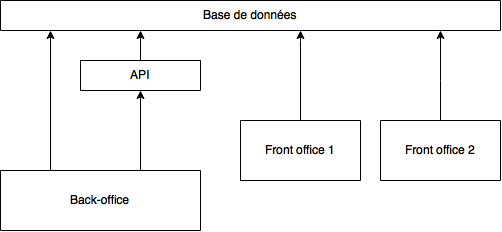
\includegraphics[scale=0.75]{images/architecture_open_orchestra}
        \end{center}
        \caption{Exemple d'architecture d'utilisation d'Open Orchestra}
        \label{architecture}
      \end{figure}

   
\section{Fonctionnalités}
	    \paragraph{}
	    Dans ce chapitre je vais vous présenter les différentes fonctionnalités d'Open Orchestra. Bien sûr, je ne vais pas tous les détailler, mais uniquement les points clés qui permettent une bonne compréhension du projet.
	      \subsection{Blocs}
	        \label{Blocs}  
	       \paragraph{}
	      Dans Open Orchestra tous les éléments visibles en front sont représentés par des blocs. Un bloc est simplement une entité avec des attributs qui varient selon le type de bloc. Chaque type de bloc sont indépendant, c'est-à-dire que eux seul connaissent leurs attributs, leurs façon de s'afficher en front ou en back-office ou encore la façon dont ils peuvent être contribué en back-office. 
	       \paragraph{}
	       Pour permettre cette indépendance, Open Orchestra utilise le design pattern stratégie. Le pattern stratégie permet de rendre une famille d'algorithmes interchangeables et ainsi  la possibilité d'exécuter un traitement spécifique selon le contexte.

          \paragraph{}
	       Comme le présente le diagramme de classe~\ref{pattern strategy} chaque bloc possède une classe qui indique comment il doit s'afficher pour cela la classe a deux méthodes, la première qui indique le bloc qu'elle supporte (\verb?support?) et la méthode \verb?show? qui fourni le rendu, d'un autre coté il y a une classe que appelé \verb?manager?  qui est la seule a connaitre toutes les stratégies des différents blocs. 
		\begin{figure}[H]
        \begin{center}
          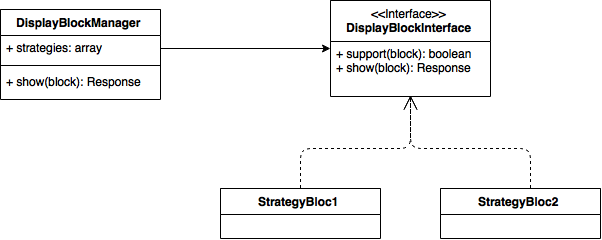
\includegraphics[scale=0.75]{images/strategy_block}
        \end{center}
        \caption{Utilisation du pattern stratégie pour l'affichage des bloc en front}
        \label{pattern strategy}
      \end{figure}
         \paragraph{}
	       Ainsi, lorsque que l'on désire afficher un bloc, il suffit de demander au manager d'afficher ce bloc, ce dernier va chercher parmi les stratégies qu'il connait laquelle supporte (méthode \verb?support?) le bloc et s'il en trouve une alors il exécute la méthode (\verb?show?) de la stratégie.
	        
	      	\paragraph{}
	      	Par défaut, le CMS propose de nombreux types blocs  comme par exemple un bloc pour lister un type de contenu, afficher un texte formaté, afficher un carrousel ou un média, un menu, une carte, un bloc de contact, etc.
	      \paragraph{}
	      	 Bien-sûr, il possible pour un intégrateur \footnote{Dans le cadre de ce rapport un intégrateur indique une personne ou une équipe qui utilise Open Orchestra afin de  l'étendre pour des besoins particuliers}, de créer son propre type de bloc, il lui suffit de développer les différentes stratégies (affichage en front et back-office, formulaire en back-office, etc) nécessaire à un bloc.  
         \subsection{Nodes}
         \paragraph{}
         Un des points central d'un CMS est les pages. Sur Open Orchestra les pages sont identifiées comme des noeuds (\og nodes \fg{}).
          Les nodes sont simplement des conteneurs qui contiennent des zones. Les zones permettent d'organiser la page, elles contiennent des sous-zones ou des blocs ce qui permet un découpage fin de la page pour simplifier sont organisation. 
         \paragraph{}
         Il existe trois types de nodes : 
         \begin{itemize}
         \item[]
         \item  Les nodes qui représentent les pages visibles en \og front \fg{}.
          \item[]
         \item  Les \og node tranverse \fg{} qui contiennent les blocs transverses, c'est-à-dire les blocs qui sont communs à plusieurs pages comme le bloc \og menu \fg{} ou encore le bloc \og footer \fg{}.
          \item[]
         \item Le dernier type de nodes sont ceux qui permettent de contribuer les pages d'erreurs (404, 503) d'un site.
         \end{itemize}
         \paragraph{}
		Le schéma~\ref{node} montre un exemple typique de page avec trois zones, le header qui contient un bloc menu, le footer un bloc footer et une zone principale découpé elle-même en deux zones avec un bloc de contact pour la zone de droite et un bloc de texte à gauche.
		\begin{figure}[H]
        \begin{center}
          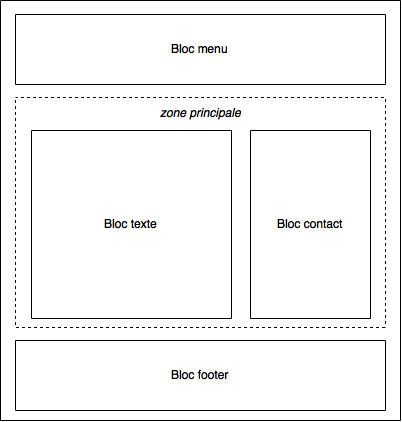
\includegraphics[scale=0.75]{images/node}
        \end{center}
        \caption{Exemple de page}
        \label{node}
      \end{figure}
         \subsection{Content type}
         Le second point important d'un CMS est les contenus avec Open Orchestra il est facile de créer des types de contenus (actualité, client, etc, ...).
          \paragraph{}
          En effet, Open Orchestra propose une approche graphique grâce à un formulaire pour créer ou éditer des types de contenus comme l'illustre la figure.
          Un type de contenu est composé de différent champs avec différente option, par exemple pour un champ de type texte il peut y avoir une option pour limiter le nombre de caractère ou encore une valeur par défaut.
          \paragraph{}
          Par défaut, Open Orchestra offre une liste de types de champs (date, texte, monnaie, média, email, entier, zone de texte riche, etc) qui comme pour tous les composants d'Open Orchestra peut être étendu par d'autre type de champ personnalisé. 
\section{Caractéristiques}
   \subsection{Performance}
   Open Orchestra a été développé pour supporter une charge de trafic importante. Pour cela le CMS exploite au niveau du front l'ESI (Edge Side Includes) couplé à un reverse proxy\footnote{Un reverse proxy est un serveur qui traite les requêtes en amont du serveur web. L'intérêt d'un reverse proxy est multiple gestion de cache, chiffrement, répartition de charge}.
   \paragraph{}
   L'ESI est un langage de balisage HTML qui permet de diviser une page en différent éléments dont les rendus sont faits dans différentes requêtes par le serveur web. Ce qui permet d'avoir un cache HTTP sur les différents éléments et ainsi rafraichir seulement les éléments obsolètes de la page et non toute la page.
   \paragraph{}
   Comme nous l'avons vu dans la section~\ref{block} sur Open Orchestra les pages sont déjà découpées en différent blocs ainsi l'utilisation de l'ESI est adapté et permet une amélioration significative des performances.
   \paragraph{}
   Si nous reprenons l'exemple de notre page (schéma~\ref{node}), le schéma~\ref{esi} présente le processus effectué par le serveur dans le cas où les blocs \verb?header? et \verb?footer? sont déjà en cache lorsqu'un utilisateur demande la page.
   		\begin{figure}[H]
        \begin{center}
          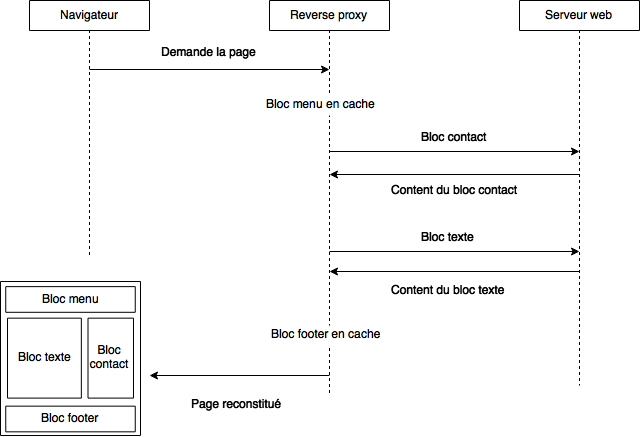
\includegraphics[scale=0.75]{images/esi}
        \end{center}
        \caption{Processus d'affichage d'une page qui utile l'ESI}
        \label{esi}
      \end{figure}
   
   \subsection{Modularités}
   Comme je vous l'expliquais en introduction la principale particularité d'Open Orchestra est sa modularité. Pour cela, les différents composants du CMS sont répartis dans différents bundles \footnote{Sous Symfony2 un bundle est un ensemble de fichiers structurés (contrôleur, entité commande, listener, formulaire) qui permettent d'implémenter une ou des fonctionnalités qui dans l'idéale peuvent être réutilisés dans différent projets}
   \paragraph{}
   \begin{itemize}
   \item \textbf{open-orchestra-base-bundle} : Classes communes au back-office et front-office
   \item \textbf{open-orchestra-base-api-bundle} : Api d'Open Orchestra
   \item \textbf{open-orchestra-base-api-mongo-model-bundle} : Implémentation des models nécessaires à l'api pour \verb?MongoDB? 
   \item \textbf{open-orchestra-cms-bundle} : Logique du back-office
   \item \textbf{open-orchestra-front-bundle} : Logique du front-office
   \item \textbf{open-orchestra-display-bundle} : Logique d'affichage des blocs en Front-office
   \item \textbf{open-orchestra-media-bundle} : Médiathèque d'Open Orchestra
   \item \textbf{open-orchestra-media-admin-bundle} : Administration de la médiathèque d'Open Orhcestra
   \item \textbf{open-orchestra-model-interface} : Interfaces des models utilisés par les autres bundles 
   \item \textbf{open-orchestra-model-bundle} : Implémentation des models pour \verb?MongoDB? 
   \item \textbf{open-orchestra-user-bundle} : Gestion des utilisateurs 
   \item \textbf{open-orchestra-workflow-function-bundle} : Système de workflow pour le back-office 
   \end{itemize}
   \paragraph{}
    Une application front-office n'a aucun intérêt à charger toute la logique du back-office ainsi grâce à ce découpage chaque application (front-office ou back-office) charge uniquement les composant qui lui est nécessaire.
   \paragraph{}
   De plus, cela permet de désactiver facilement une fonctionnalités. Par exemple, si un intégrateur n'a pas bessoin de gérer des médias il peut alors désactiver la médiathèque en n'utilisant pas les bundles (\verb?open-orchestra-media-bundle? et \verb?open-orchestra-media-admin-bundle?).

   \paragraph{}
   Un autre avantage est la facilité de remplacement d'un composants. Par défaut Open Orchestra utilise \verb?MongoDB? comme système de gestion de base de données, mais si un intégrateur veut utiliser un autre système comme \verb?Mysql? alors il lui suffit d'écrire son propre \newline  \verb?open-orchestra-model-bundle? qui utilise bien-sûr les différentes interfaces de  \newline  \verb?open-orchestra-model-interface? adapté a \verb?Mysql?.
\part{Organisation du développement}
\chapter{Organisation du développement}
Introduction, pas eu de tâche particulière intégration au sein de l'équipe avec diff tâches (ajout fonctionnalités, correction bug, Documentation en aglais, refacto, optimisation, formation

\section{Gestion de projet agile}
\subsection{Méthodes agiles}
\paragraph{}
Le projet a été mené selon une approche agile. La gestion de projet agile repose sur un développement itératif qui consiste à découper un projet en plusieurs itérations appelé sprint. Les méthodes agiles définis plusieurs valeurs fondamentales : 
\begin{itemize}
\item La communication au sein de l'équipe
\item La collaboration avec le client, celui-ci doit être impliqué tous au long du développement.
\item L'adaptation au changement, c'est-à-dire que le planification initiale doit être flexible pour permettre l'évolution de la demande. 
\end{itemize}
Il existe différentes type de méthode agile (Scrum, XP, RAD...) qui possèdent leurs propres caractéristiques.
\paragraph{}
Pour le développement d'Open Orchestra, c'est la méthode Scrum qui est utilisé. Scrum définis trois rôles au sein d'une équipe : 
\begin{itemize}
\item  Le \og Product Owner (PO) \fg{} qui porte la vision du produit
\item Le \og Scrum Master \fg{} est le responsable de la mise en œuvre de la méthode, il doit s'assurer que cette dernière est correctement appliqué
\item L'équipe de développement qui est chargé de transformer les besoins exprimés par le Product Owner. 
\end{itemize}
\paragraph{}
La réalisation d'un projet utilisant la méthode est rythmée par différents évènements : 
\paragraph{}
Tous d'abord, le sprint qui est représente une période de courte durée, de une à quatre semaines, durant laquelle l'équipe effectue un nombre de tâches définis à l'avance.
 \paragraph{}
 La réunion de planification où l'équipe répond à deux questions, \og Quoi ? \fg{} c'est-à-dire les tâches du backlog\footnote{Le backlog est un ensemble de fonctionnalités ou de tâches nécessaire pour la réalisation satisfaisante d'un projet} qu'elle réalisera au prochain sprint et \og Comment ? \fg{} c'est a ce moment que l'équipe estime les tâches choisis au \og Quoi \fg{} 

 \paragraph{}
Le \og daily scrum \fg{} qui est une réunion réalisé quotidiennement. Durant cette réunion chaque membre de l'équipe indique les tâches qu'il a réalisé depuis le dernier daily et celles qu'il va effectuer jusqu'au prochaine daily et pour finir les difficultés qu'il a ou pense rencontrer.
Cette réunion permet à tous les membres de connaître les tâches de chacun afin de s'entraider et d'anticiper plus facilement les obstacles.
 \paragraph{}
Pour finir à la fin du sprint, les membres de l'équipe se réunisse pour la revue de sprint durant laquelle les différentes tâches réalisés durant le sprint sont présentés et validés. Puis pour la rétrospective qui permet de mettre en évidence les points positif et les actions a mettre en place pour améliorer le prochain sprint.

SCHEMA (schéma sprint)
\subsection{Scrum avec Open Orchestra}
Au sein du projet Open Orchestra, la méthode Scrum est appliqué.. Ainsi des sprint de une semaine avec un daily scrum tous les jours a midi.
De plus, tous les mercredis ou mardis selon les disponibilités une \og cérémonie \fg{} qui comprend la réunion de planification et la rétrospective.
Concernant, la revue de sprint (validation des taches du sprint) celle-ci n'est pas faite durant une réunion définis mais tout au long du sprint par le product ownver.
 \paragraph{}
 Pour faciliter la mise en place de la méthode Scrum, l'équipe utilise différent outils.
 Tous d'abord Skype et Slack\footnote{Slack est une plateforme de communication réalisé en 2014 qui permet d'intégrer facilement différents outils de service en ligne tel que github, trello, dropbox, google drive, ...)} pour la communication.
  \paragraph{}
 Et enfin Trello pour organiser les tâches, en effet l'équipe possédé un \verb?board? avec différentes colonnes pour organiser les tâches : 
 \begin{itemize}
 \item[]
 \item \textbf{Backlog} : le backlog qui contient les différentes tâches a effectué pour le projet, le tâches du backlog sont organisées en quatre colonnes (Nice to have, Good, Great, Must have) selon la priorité de la tâche.
 \item \textbf{Support} : Les demandes effectué par les différentes équipes d'intégrateur d'Open Orchestra au sein d'Interakting.
 \item \textbf{Proposition} : Les différentes propositions d'amélioration ou de re- factorisation du code faites par les membres de l'équipe.
 \item \textbf{Bugs} : Les différents bug rencontrés durant le développement
 \item \textbf{Todo} : Les taches a effectuer durant le sprint en cours.
 \item \textbf{Doing} : Les taches actuellement en développement.
 \item \textbf{Blocked} : Les taches bloqué pour différentes raison (manque de précision de la tache, bug empêchant la réalisation de la taches)
 \item \textbf{ToDeploy} : Taches réalisés qui sont prêtes a être déployé sur le serveur d'intégration.
 \item \textbf{ToValidate} : Taches du sprint en attente de validation par le product owner.
 \item \textbf{Failed} : Taches du sprint e non validé par le product owner
 \item \textbf{Done} : Taches du sprint validé par le product owner
 \item[]
 \end{itemize}
Les colonnes \verb?ToDeploy?, \verb?Done? sont unique a un sprint, il y a donc une colonne  différent\verb?ToDeploy?, \verb?Done? pour chaque sprint.
\paragraph{}
Par exemple, une tâches suit un processus, présenté par le schéma, bien particulier entre l'intrégration de la tache dans la sprint et ca validation par le product ownver. Ce processus permet de suivre facilement l'avancement ou encore les différents problèmes rencontrés sur les différentes tâches par tous les membres de l'équipe.
\section{Intégration continue}
Pour le dévellopement d'Open Orchestra les principes de l'intégration continue sont utilisés. 
\begin{quotation}
L'intégration continue est un ensemble de pratiques utilisées en génie logiciel consistant à vérifier à chaque modification de code source que le résultat des modifications ne produit pas de régression dans l'application développée.
\end{quotation}
L'utilisation de ces pratiques apporte de nombreux avantages, tous d'abord comme il est indiqué dans la citation cela permet de minimiser les régréssions mais aussi d'avoir a tous moment un produit (logiciel, site, etc) utilisable.
\paragraph{}
La mise en place de cette technique nécéssite différentes pré-requis : 
\begin{itemize}
\item[]
\item Dépot unique de code source versionné
\item Automatisation des tests
\item Un environnement similaire a celui de production
\item Automatiser le deploiement
\end{itemize}

\subsection{git}
Dans le cadre d'Open Orchestra, le code source est versionné avec git\footnode{Git est un lgociel de versionning décentralisé, c'est-à-dire qu'il n'existe pas un dépôt unique mais un dépot local pour chaque développeurs.} et utilise GitHub qui est un service web permettant d'heberger un dépôt git. Comme je l'expliquais lors des présentations des caractèristiques d'Open Orchestra, ce dernier est découpé en plusieurs bundles et donc chaque bundles posséde son propre dépôt sur GitHub.
\paragraph{}
Open orchestra étant toujours en version béta, il n'y a pas de realease a proprement parlé. Ainsi le worklow de dévellopement sur github est simplifié car il n'y a qu'une seule branche stable, la branche maste. Les autres branches sont des branches temporaires d'ajout de fonctionnalités ou de correction de bugs. Ce type de workflow est appellé \verb?GitHub flow? et est représenté par le schéma.
\paragraph{}
Ainsi avec ce type de workflow, la modification du code source que ce soit pour corriger un bug ou ajouter une fonctionnalités s'effectue toujours de la même manière : 
\begin{enumerate}
\item[]
\item Mettre à jour sa branche master en local
\item Créer une nouvelle branche en local à partir de master
\item Effectuer les modifications dans cette branche
\item Pousser sa branche sur GitHub (origin)
\item Vérifier que les tests fonctionnne, je reviendrais plus en détail sur ce point par la suite
\item Ouvrir une pull-request, sur GitHub une pull-request consiste à faire une proposition de modification, à partir de cette pull-request les différents membres peuvent commenter, valider ou non la modification.
\end{itemize}

Une fois la pull-request validé, elle peut être mergé avec master, c'est-à-dire inclure la modification dans la branche master.
\paragraph{}
Lorsqu'une branche est poussé sur l'un des dépôts GitHub du projet, les tests sont automatiquement lancé. Pour cela, les différents dépôts du projet intégre un outil \verb?Travis CI?. Travais CI 

Pour eviter au maximun les régréssion utilsiation de travis description plus tard)
Plate forme d'integration (la ou valide le PO), un déploiement plusieurs fois par jour sur l'environnement prod) utililisation capistrano ( présentation de l'outil) 
Deploiement (capistrano)
\section{Qualité}
PSR2 (qu'est ce que c'est, présentation)
code climate (outil qui vérifie la qualité du code et fournis une note) 
SensioInsignt (Outil de qualite d'application Symfony)
Travis, (Détail a quoi ça sert, comment cela fonctionne (hook github lancement des test) 
Test unitraite, Test fonctionel, (Mise en place de test  pour tous les codes metiers) 
Behat (mise en place de test behat) 

\newpage

%récupérer les citation avec "/footnotemark"
\nocite{*}

%choix du style de la biblio
\bibliographystyle{plain}
%inclusion de la biblio
\bibliography{bibliographie.bib}
%voir wiki pour plus d'information sur la syntaxe des entrées d'une bibliographie

\end{document}